\documentclass[a4paper, 12pt]{article}
\usepackage[top=2cm, bottom = 2cm, left = 2cm, right = 2cm]{geometry}
\usepackage[utf8]{inputenc}
\usepackage[brazil]{babel}
\usepackage{listings}
\usepackage[framed, numbered]{matlab-prettifier}
\usepackage[T1]{fontenc}
\usepackage{indentfirst}
\usepackage{graphicx}
\usepackage{epstopdf}
\usepackage{float}
\usepackage{amsmath}
\usepackage{amssymb}
\usepackage{systeme}

\title{Relatório do Laboratório 2 - Teorema da Amostragem \\ EET-01}

\author{
  Igor Magalhães\\igorcmag@gmail.com
  \and
  Rafael Gonçalves\\rafael.goncalves@ga.ita.br
}
\date{23 de maio de 2020}

\begin{document}
\maketitle
\section{Aliasing de um Senoidal}

\subsection{a)}
oi
%\lstinputlisting[style=Matlab-editor, caption={Código em MATLAB para gerar as quatro sequências do item (a) do exercício 1, bem como a plotagem dos seus respectivos gráficos.}, basicstyle = \mlttfamily\scriptsize]{../Programas/ex1/a.m}

%\begin{figure}[H]
%	\centering
%	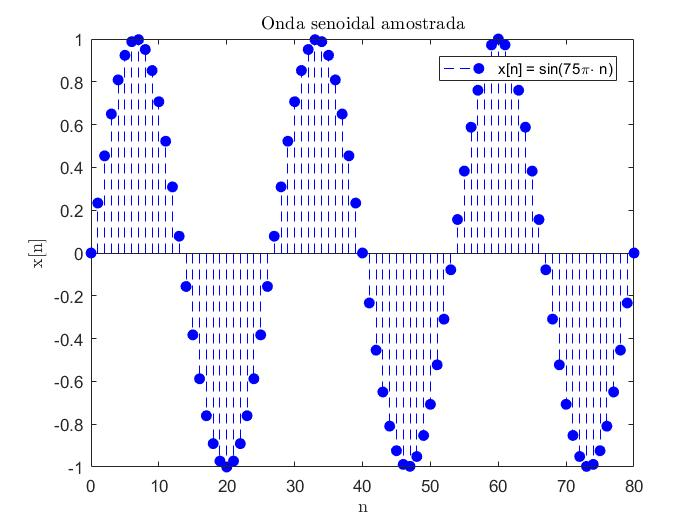
\includegraphics[scale=0.7]{../Imagens/ex1/a.jpg} 
%	\caption{Gráficos das sequências em seus respectivos domínios}
%	\label{fig:1a}
%\end{figure}

\subsection{b)}

\subsection{c)}

\subsection{d)}

\subsection{e)}

\section{Aliasing de um Chirp}

\subsection{a)}

$$f_i(t)=\mu t+f_l=600t+4 \therefore f_i(0)=4kHz \therefore f_i(50ms)=600\cdot 0.05+4=34kHz$$
Assim, a faixa de frequência é de $0$ a $34kHz$.

\subsection{b)}

$$c[n]=c(nT)=c(\frac{n}{f_s})=cos(\frac{\pi \mu}{{f_s}^2}n^2 + \frac{2\pi f_l}{f_s}n + \psi)$$

Fazendo $f_s=8kHz$ e $\psi=0$:

$$c[n] = cos(\frac{3}{320}\pi n^2 + \pi n)$$

Perceba que a função é par. O sinal de amostragem foi gerado pelo \textbf{código} e seu gráfico está exposto na \textbf{figura}. 

\lstinputlisting[style=Matlab-editor, caption={Código em MATLAB para gerar o sinal amostrado do item (b) do exercício 2, bem como seus gráficos 'plot' e 'stem'.}, basicstyle = \mlttfamily\scriptsize]{../Programas/ex2/b.m}

\begin{figure}[H]
	\centering
	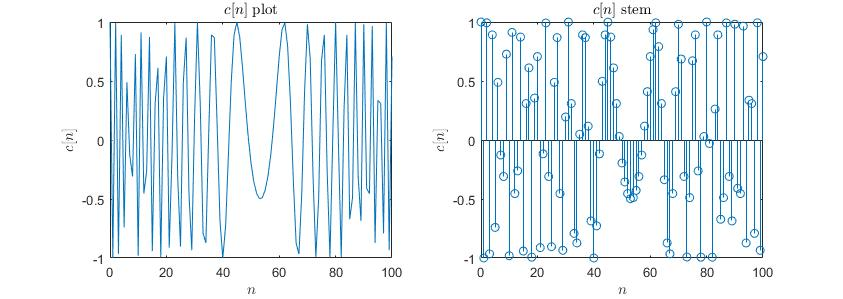
\includegraphics[scale=0.6]{../Imagens/ex2/b.jpg} 
	\caption{Gráficos 'plot' e 'stem', respectivamente, de $c[n]$}
	\label{fig:1a}
\end{figure}

\subsection{c)}

$$f_i(t) = 0 \therefore \frac{\mu}{{f_s}^2}n + \frac{f_l}{f_s} = 0 \therefore n\approx -53$$.

Isso é confirmado pelo gráfico, pois a função é par, isto é, $f(-n)=f(n)$, podemos olhar em $n=53$. No tempo, isso equivale a $t=\frac{n}{f_s}=6.67ms$. No \textbf{código}, plotamos $c[n]$ para $n$ de $0$ a $1000$, como mostra a \textbf{figura}. Vemos que as regições de baixa frequência estão regularmente espaçadas.

\lstinputlisting[style=Matlab-editor, caption={Código em MATLAB para gerar o sinal amostrado do item (b) do exercício 2, bem como seu gráfico 'plot' para n variando de 0 a 1000.}, basicstyle = \mlttfamily\scriptsize]{../Programas/ex2/c.m}

\begin{figure}[H]
	\centering
	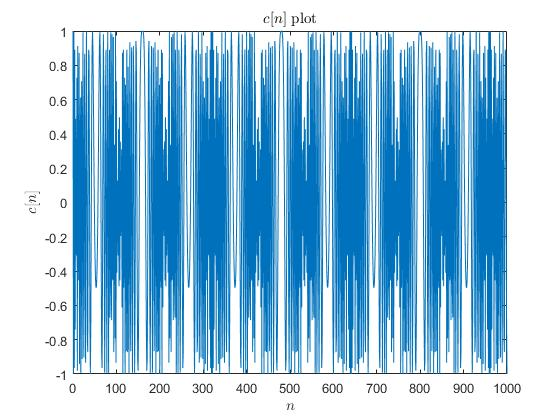
\includegraphics[scale=0.6]{../Imagens/ex2/c.jpg} 
	\caption{Gráfico 'plot' de $c[n]$ com $n$ de $0$ a $1000$}.
	\label{fig:1a}
\end{figure}

\section{Escutando o Aliasing}

\subsection{a)}

\subsection{b)}

\section{Montagem de uma Onda Sinoidal}

As equações são:
$$2=Acos(\phi)$$
$$1=Acos(\omega +\phi)$$
$$-1=Acos(2\omega +\phi)$$

Somando a segunda com a terceira, tem-se:

$$Acos(\omega +\phi) + Acos(2\omega +\phi) = 0 \therefore cos(\frac{3\omega}{2} + \phi)cos(\frac{\omega}{2})=0$$

$$cos(\frac{\omega}{2})=0 \therefore \omega = (2k+1)\pi, $$

ou

$$cos(\frac{3\omega}{2} + \phi)=0 \therefore \omega = \frac{(2k+1)\pi}{3} - \frac{2\phi}{3}.$$

Substituindo $A$ da primeira equação na segunda, tem-se

$$\frac{1}{2}cos(\phi)=cos(\omega + \phi).$$

No primeiro caso, $cos(\omega + \phi)=cos((2k+1)\pi + \phi)=-cos(\phi)$, logo $\frac{1}{2}=-1$, absurdo. No segundo caso

$$\frac{1}{2}cos(\phi) = cos(\frac{2(k+1)\pi}{3} + \frac{\phi}{3})$$

A resolução analítica desta equação é complicada e depende do resto que $k$ deixa na divisão por $3$, isto é, é preciso separar em três casos. Para mostrar que não há uma única solução, é suficiente darmos um contra-exemplo. 

Para $k=1$, temos a solução $\phi=\pi$ no intervalo $[0, 2\pi).$ A solução final fica

$$x_1(t)=-2cos(\frac{\pi}{3}t + \pi)=2cos(\frac{\pi}{3}t)$$

Para $k=4$, temos a mesma equação em $\phi$ e portanto a mesma solução $\phi=\pi$. No entanto, dessa vez a solução final fica

$$x_2(t)=-2cos(\frac{7\pi}{3}t + \pi)=2cos(\frac{7\pi}{3}t)$$

Portanto, a informação não é suficiente para determinar $x(t)$.

\section{Interpolação Polinomial Linear}

\subsection{a)}

\subsection{b)}

\subsection{c)}

\section{Filtragem Passa-Baixo Ideal}

\subsection{a)}

No \textbf{codigo}, implementamos a função \textit{interpolador-seno}, que recebe o vetor $x$ de amostras, o vetor $n$ dos índices correspondentes, e o período de amostragem $T_s$. Ele então reconstrói o sinal contínuo $x_r$ dado por

$$x_r(t) = \sum_{i=1}^{length(n)}x[i]\frac{sin(\pi (t - n[i]T_s)/T_s)}{\pi (t - n[i]T_s)/T_s}$$ 

\lstinputlisting[style=Matlab-editor, caption={Código em MATLAB que cria a função interpoladora senoidal.}, basicstyle = \mlttfamily\scriptsize]{../Programas/ex6/interpolador_seno.m}

\subsection{b)}

Usamos a função criada para interpolar uma amostra de um único ponto $x(0)=1$, como descrito no \textbf{codigo} e exposto na \textbf{figura}.

\lstinputlisting[style=Matlab-editor, caption={Código em MATLAB interpolar a amostra de um único ponto x(0)=1, bem como plotar seu gráfico.}, basicstyle = \mlttfamily\scriptsize]{../Programas/ex6/b.m}

\begin{figure}[H]
	\centering
	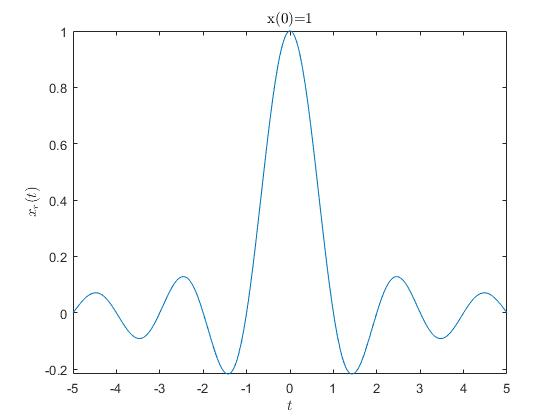
\includegraphics[scale=0.6]{../Imagens/ex6/b.jpg} 
	\caption{Gráfico da interpolação senoidal da amostra de um único ponto $x(0)=1$}.
	\label{fig:1a}
\end{figure}

\subsection{c)}

Dessa vez usamos a função criada para interpolar uma amostra de três pontos $x(0)=2$, $x(1)=1$ e $x(2)=-1$ como descrito no \textbf{codigo} e exposto na \textbf{figura}.

\lstinputlisting[style=Matlab-editor, caption={Código em MATLAB interpolar a amostra de três pontos $x(0)=2$, $x(1)=1$ e $x(2)=-1$, bem como plotar seu gráfico.}, basicstyle = \mlttfamily\scriptsize]{../Programas/ex6/c.m}

\begin{figure}[H]
	\centering
	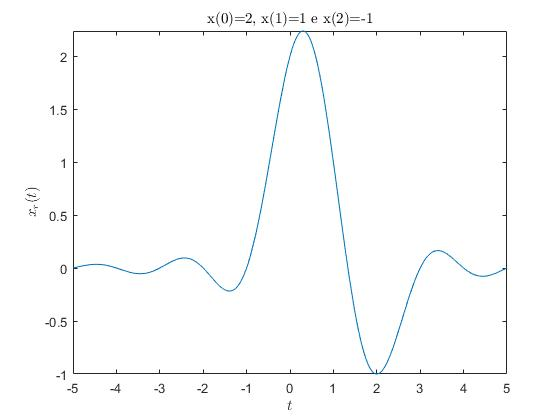
\includegraphics[scale=0.6]{../Imagens/ex6/c.jpg} 
	\caption{Gráfico da interpolação senoidal da amostra de três pontos $x(0)=2$, $x(1)=1$ e $x(2)=-1$}.
	\label{fig:1a}
\end{figure}

Perceba que o gráfico da \textbf{figura} é um ajuste do gráfico da \textbf{figura}, de modo que este passe pelos pontos amostrados.

\end{document}